\newpage
\subsection{Учет отходов производства (макулатуры)}


Макулатура собирается в прессах. Весы стоят на прессах. Оператор на прессах собирает макулатуру в тюк. Оператор фиксирует количество тюков в журнале (рис. \ref{pic:0 журнал на прессе}) и прикрепляет к каждому тюку ярлык  (рис. \ref{pic:4.19 этикетка для макулатуры_0001}). В конце смены оператор сообщает начальнику смены количество тюков макулатуры произведенных за смену, но начальник смены данные не фиксирует. Каждый тюк макулатуры принимает кладовщик, записывает в журнал.  
% (форма \ref{pic:d32}).


В системе 1С:УПП кладовщик создает документ перемещения товаров с производства на склад сырья.


%Вся макулатура в виде отходов производства передается в пресс. Кладовщик взвешивает получившийся после пресса тюк макулатуры, маркером пишет вес и водитель погрузчика перемещает тюки в   специально отведенное для хранения место. 

% Техник по учету каждый день учитывает макулатуру с пресса (рис. \ref{pic:d20}). 
% В конце месяца итоговый отчет по приемке макулатуры техник по учету передает в бухгалтерию предприятия.
Бухгалтер на его основании ставит макулатуру на приход в системе 1С:УПП. 

Макулатура продается покупателям для переработки.

\textbf{Отгрузка макулатуры}

Отгрузка макулатуры как ГП через распоряжение на отгрузку.




\textbf{Учет брака}

Учет брака на производстве не ведется.
Брак на складе в производство не возвращаются. 

\clearpage

% Мастер смены смотрит по наполнению, заказывают фуру и отгружает по мягкой накладной. Могут отвозить на другую площадку газелью и оттуда уже отгружать на продажу.
% Вся макулатура с обеих цехов привозится на пресс.
% В макулатурном прессу ведется журнал учета макулатуры (рис. \ref{pic:photo19}). На тюки крепится ярлык с весом и числом. При отгрузке макулатуры на склад выписывается форма (рис.  \ref{pic:pic_a33_1}), т.ж. каждый день подаются сведения в Отдел ГОГП (рис.  \ref{pic:pic_a34}).


% %  êîíöå ñìåíû ïðåñîâùèê ôîðìèðóåò îò÷åò (ñì. ôîðìó ''Îò÷åò ïî çàïðåñîâàííîé ìàêóëàòóðå çà ñìåíó'' \ref{pic:WasteReport2}). Îò÷åò ïåðåäàåòñÿ ìàñòåðó ïðîèçâîäñòâà.
\begin{figure}
\begin{center}
  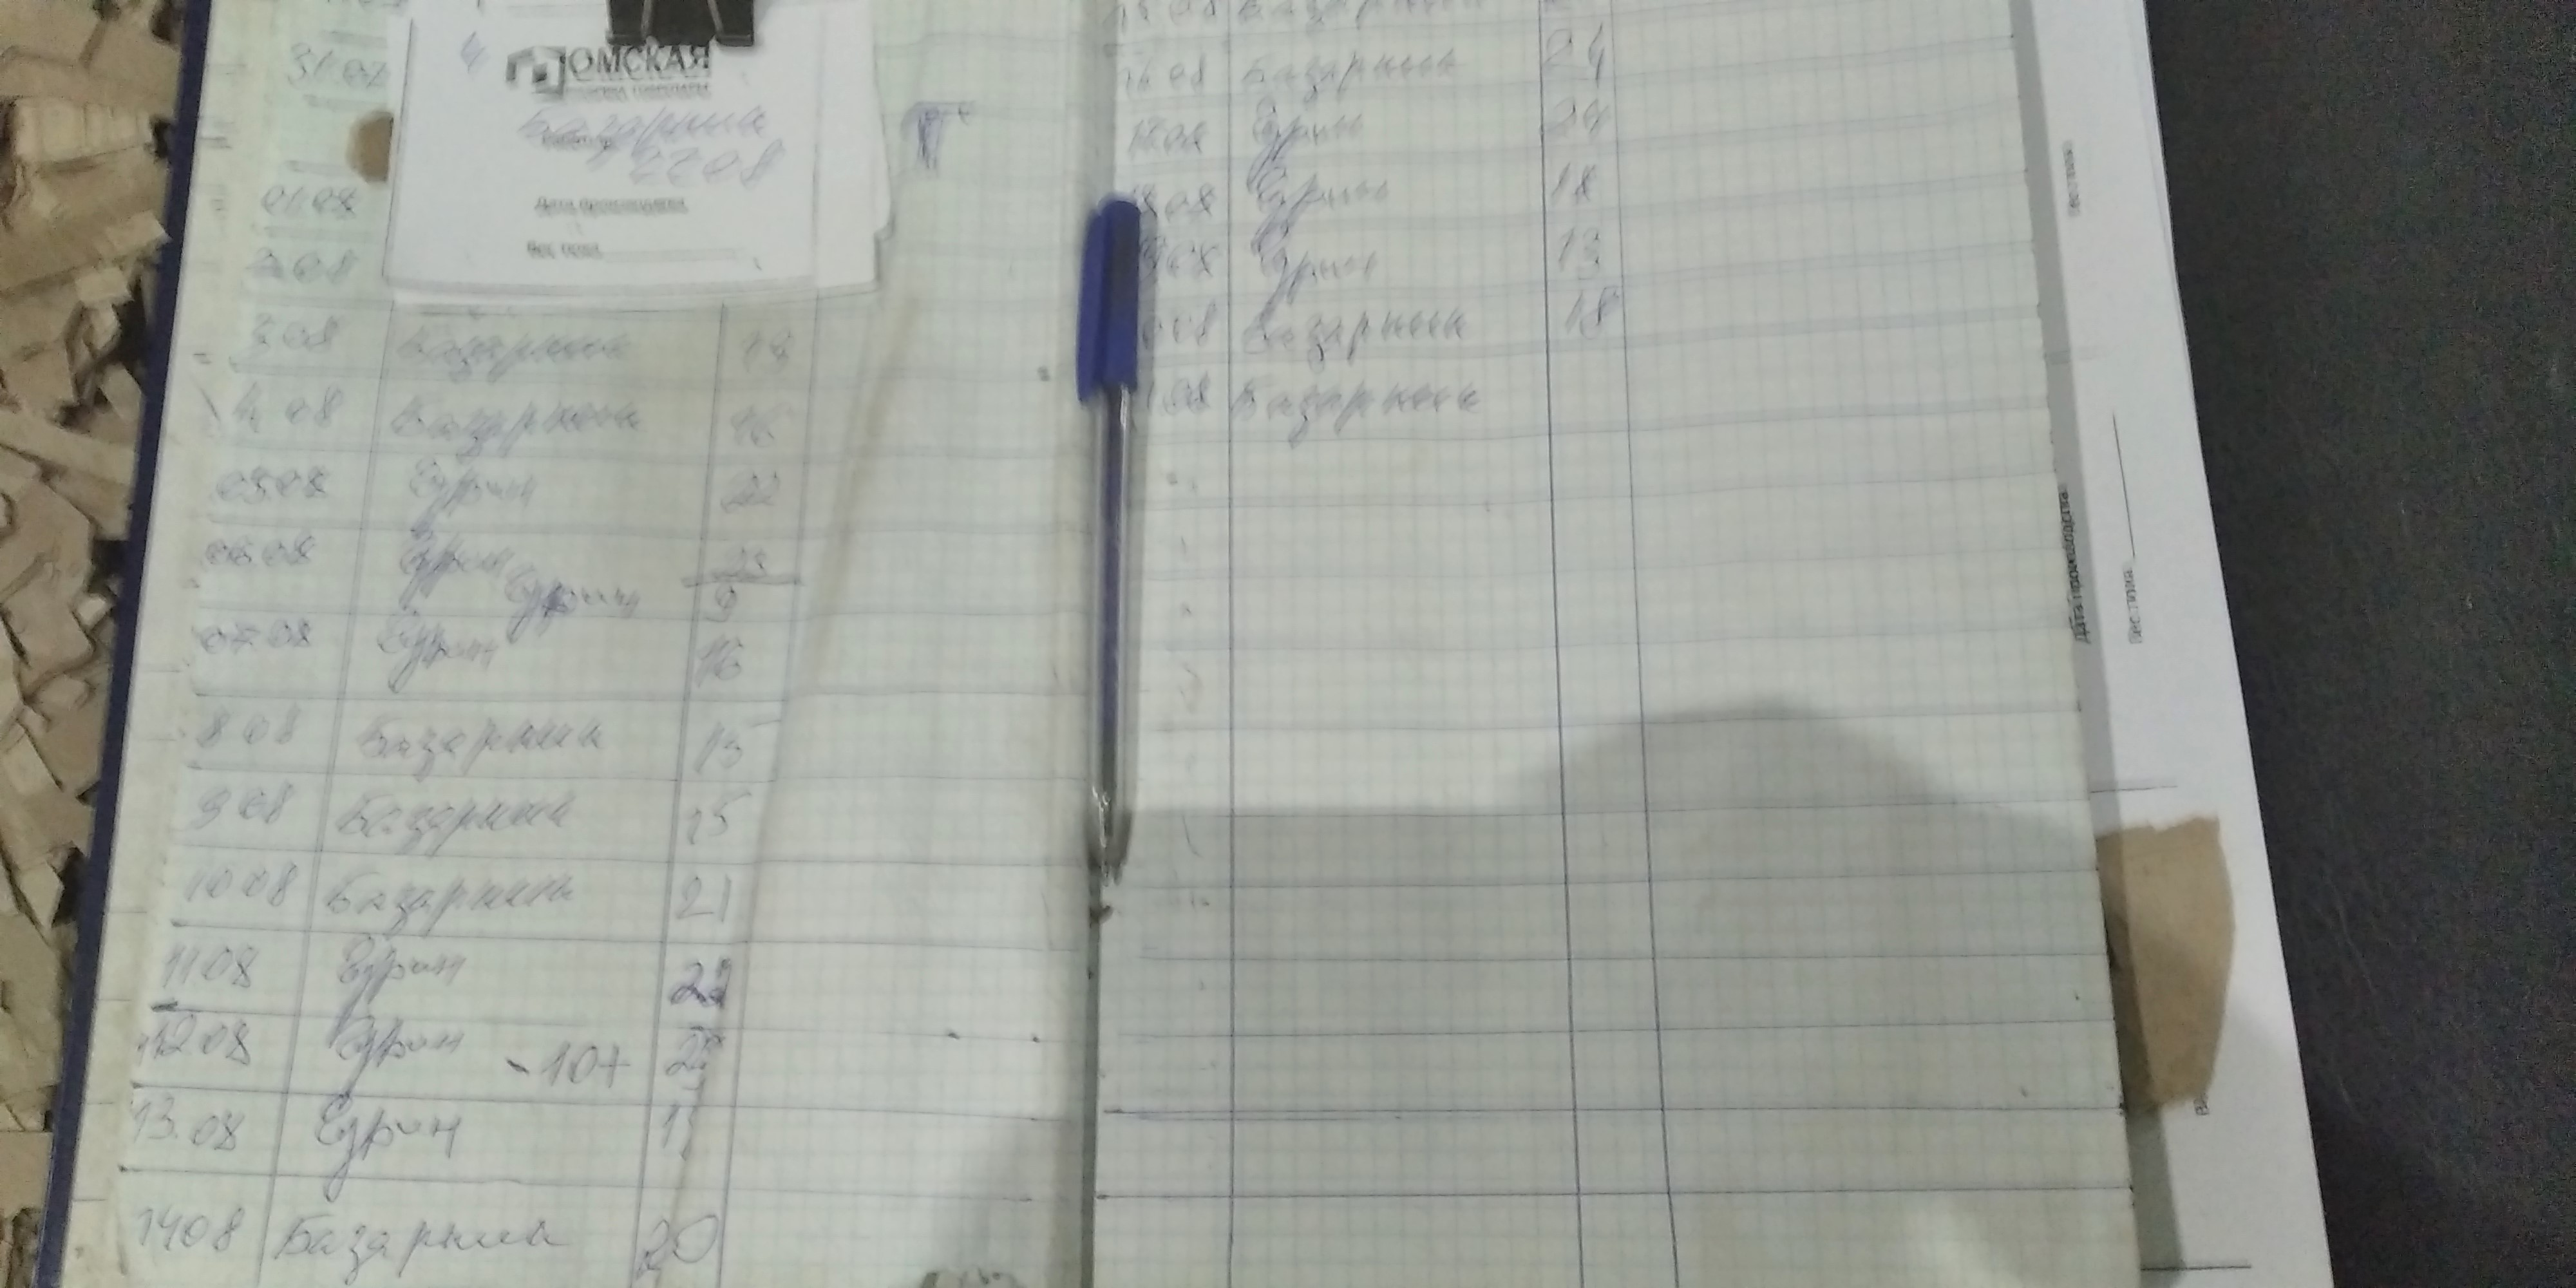
\includegraphics[height=0.94\textheight, width=0.94\textwidth, keepaspectratio]{Pics 1/0 журнал на прессе.jpg}
\end{center}
  \caption{Журнал оператора пресса}
  \label{pic:0 журнал на прессе}
\end{figure}

\begin{figure}
\begin{center}
  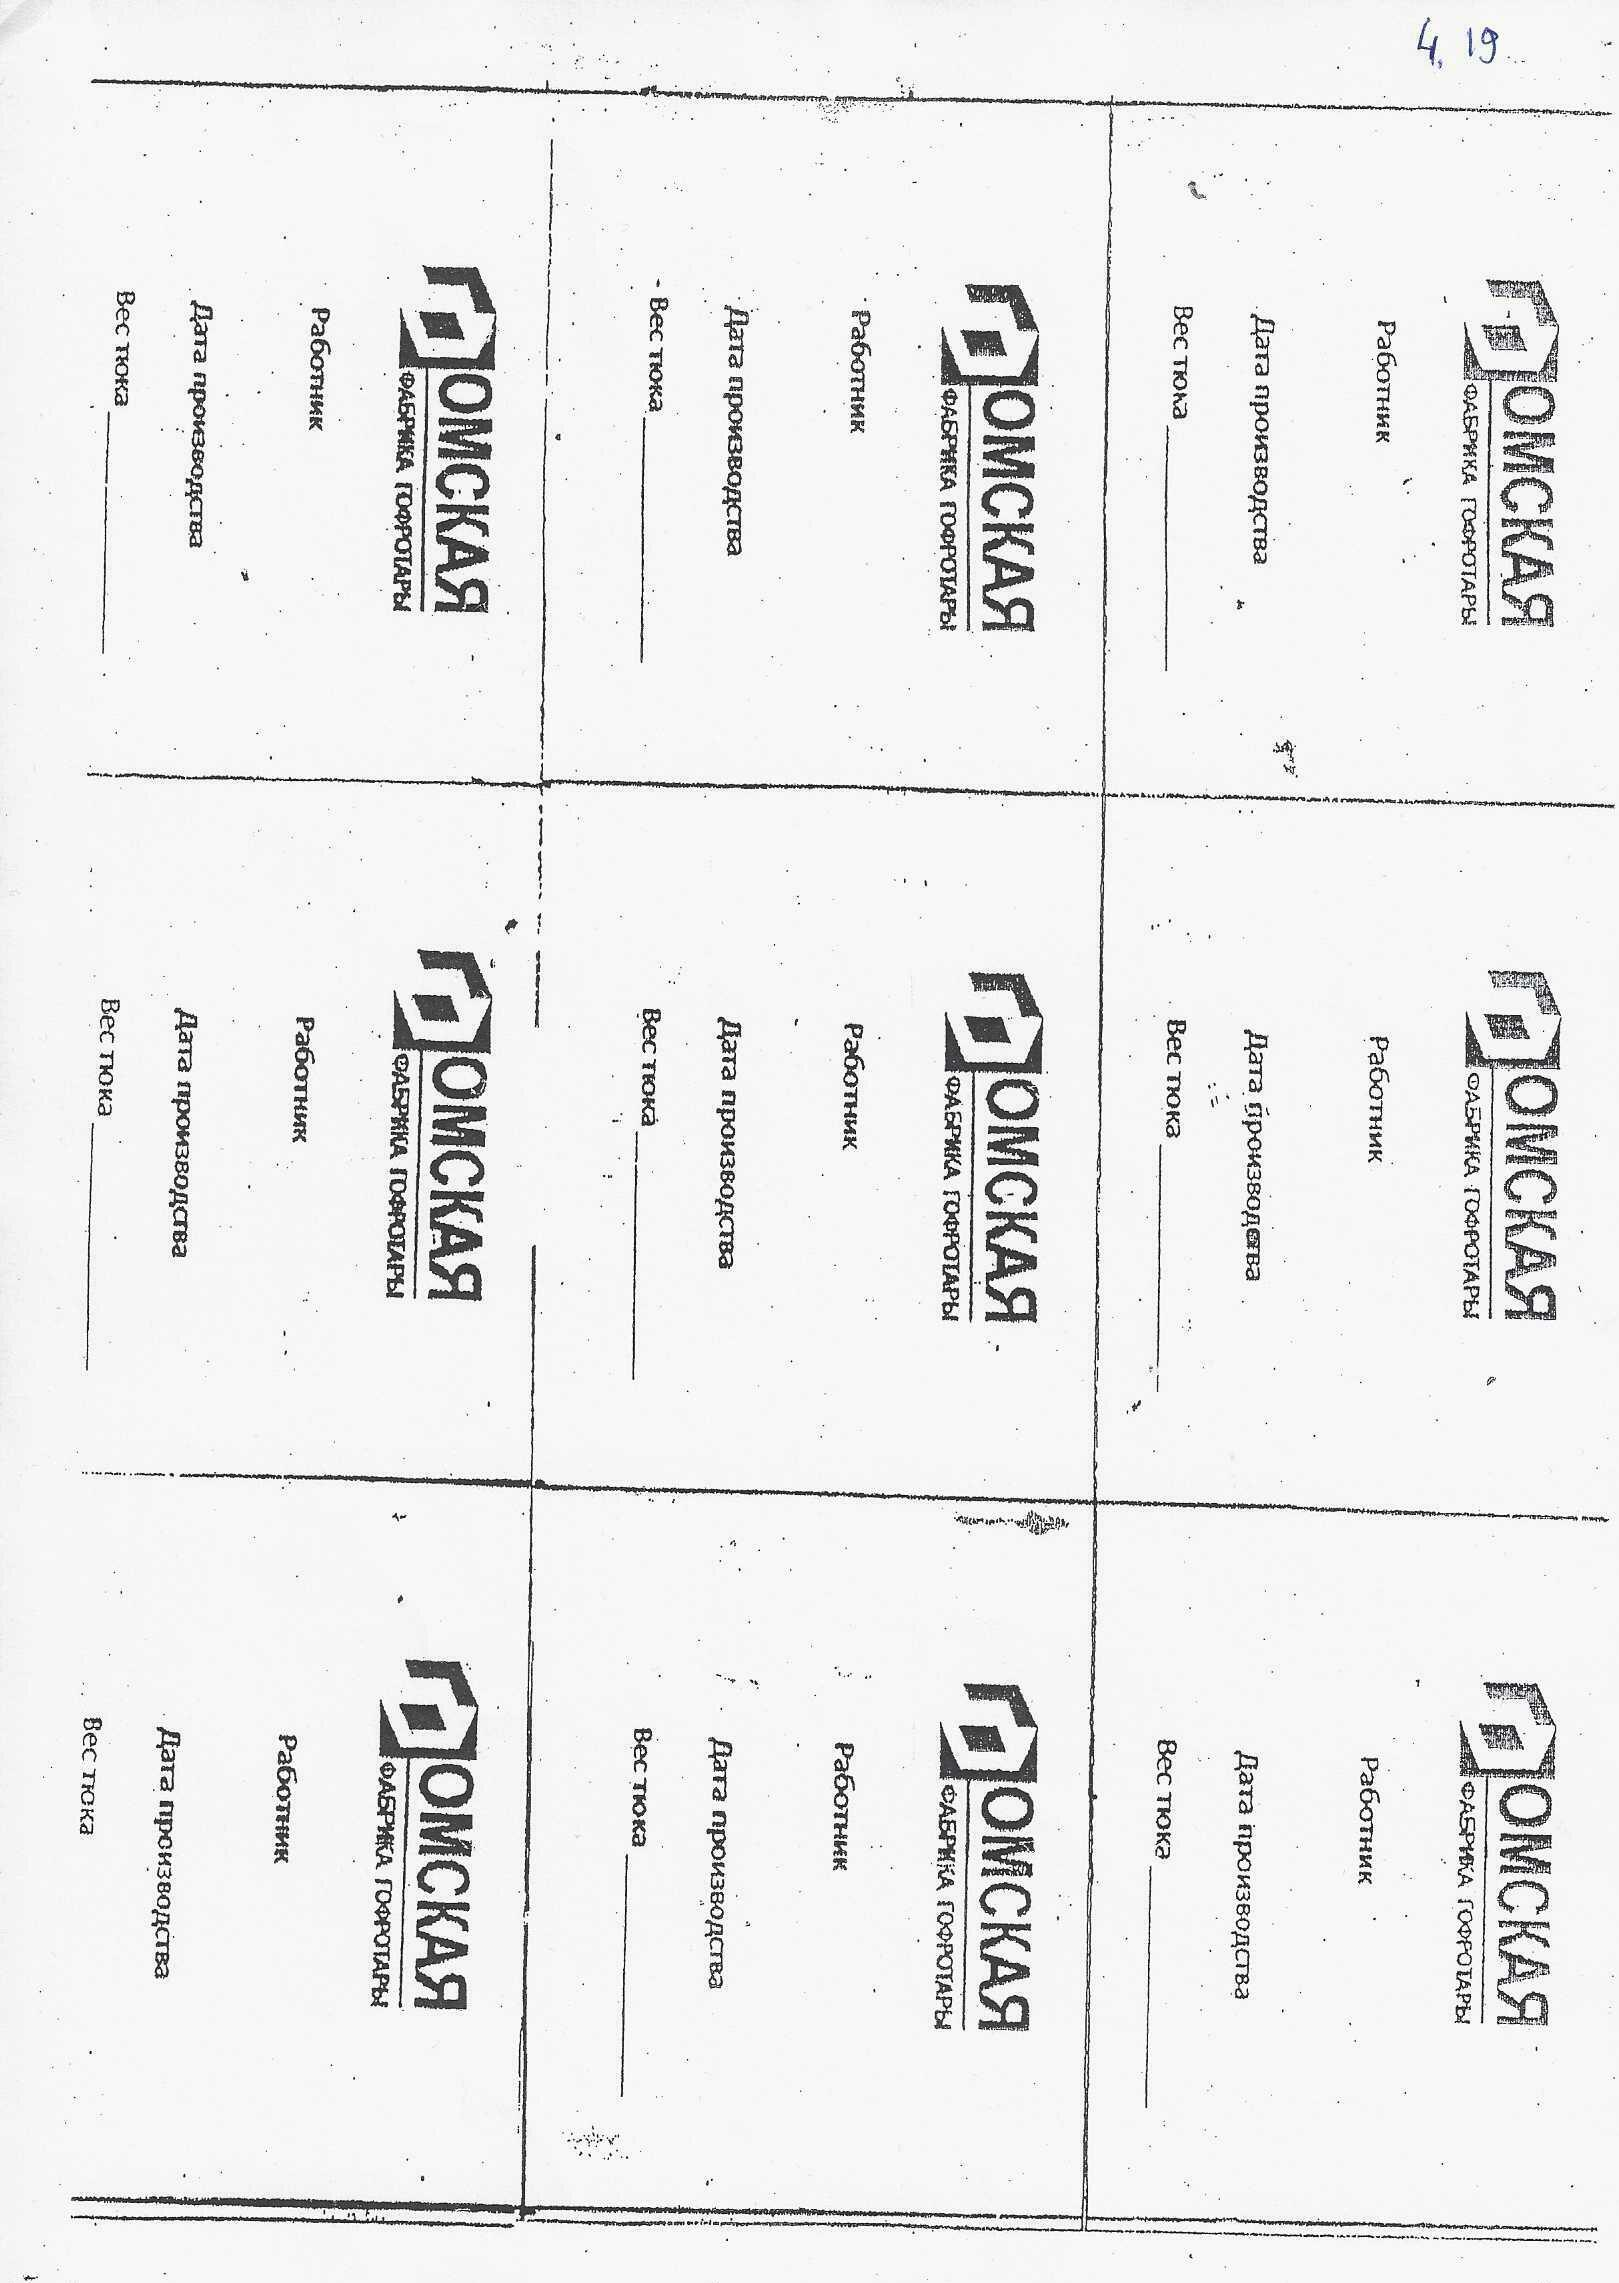
\includegraphics[height=0.94\textheight, width=0.94\textwidth, angle=180, keepaspectratio]{Pics 1/4.19 этикетка для макулатуры_0001.jpg}
\end{center}
  \caption{Ярлык для макулатуры}
  \label{pic:4.19 этикетка для макулатуры_0001}
\end{figure}
% \begin{figure}
% \begin{center}
%   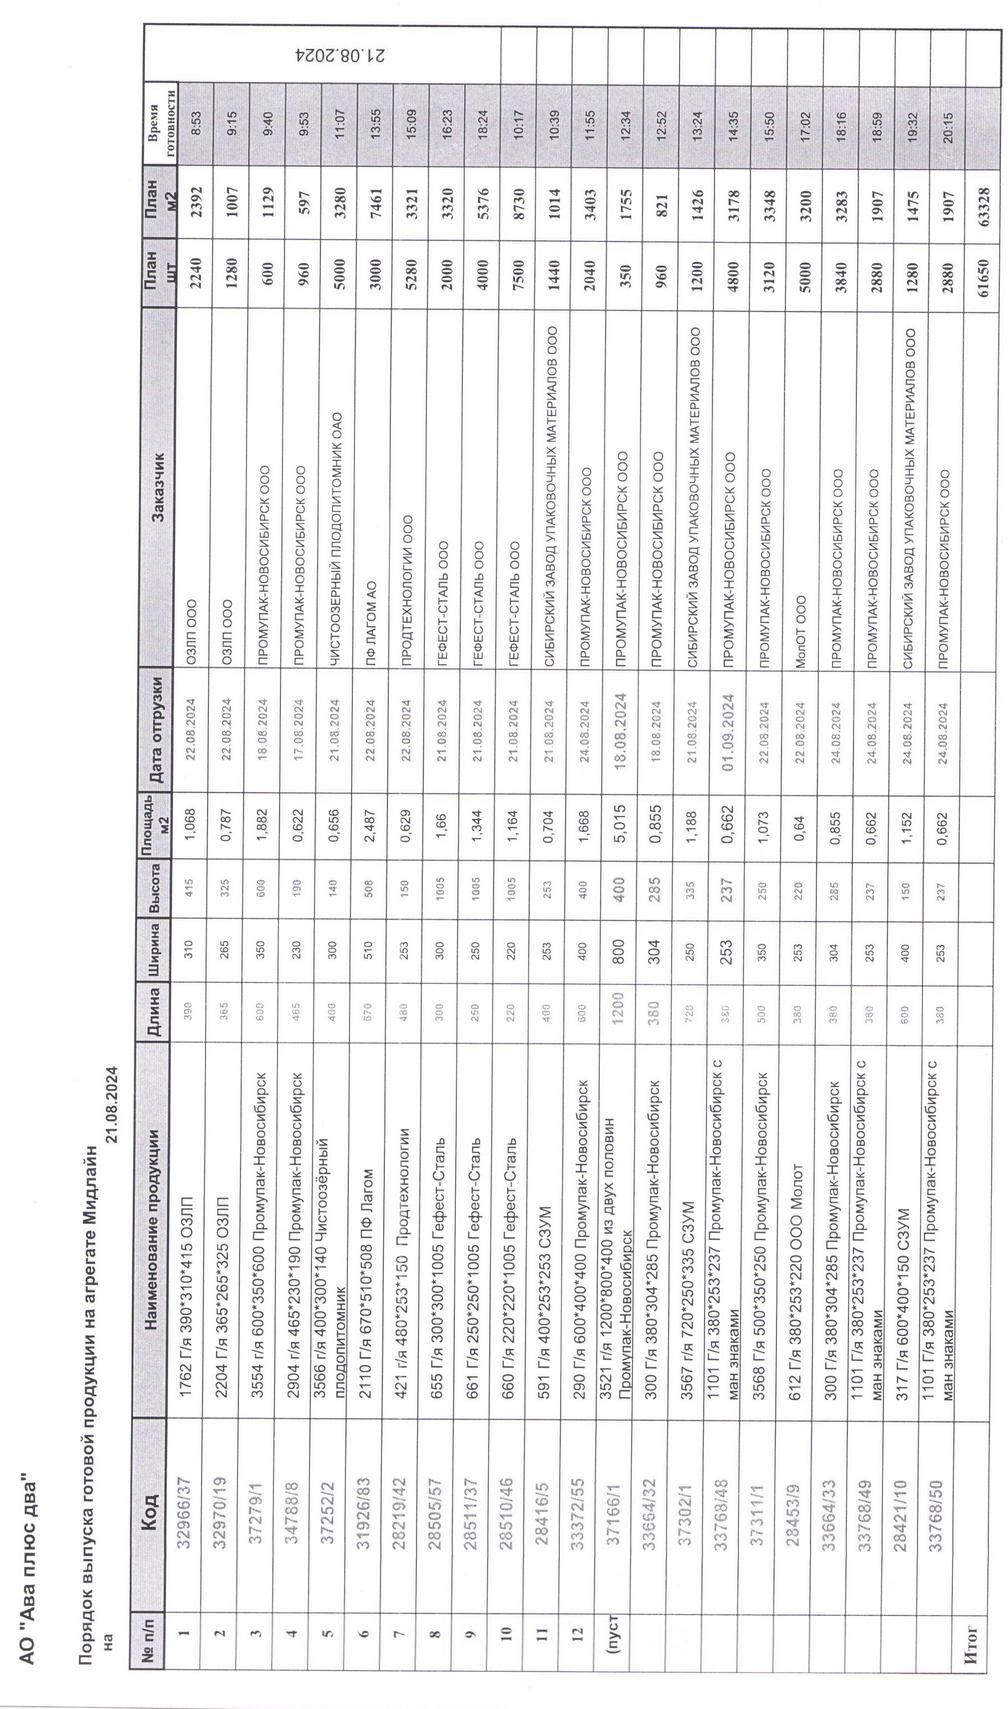
\includegraphics[height=0.6\textheight, keepaspectratio]{Pics/d20.jpg}
% \end{center}
%   \caption{Журнал учета макулатуры}
%   \label{pic:d20}
% \end{figure}
% \clearpage

% \begin{figure}
% \begin{center}
%   \includegraphics[height=0.6\textheight, keepaspectratio]{Pics/pic_a33_1.jpg}
% \end{center}
%   \caption{Рапорт по отгрузке макулатуры}
%   \label{pic:pic_a33_1}
% \end{figure}
% \clearpage

% \begin{figure}
% \begin{center}
%   \includegraphics[height=0.6\textheight, keepaspectratio]{Pics/pic_a34.jpg}
% \end{center}
%   \caption{Рапорт машиниста по макулатуре}
%   \label{pic:pic_a34}
% \end{figure}
% \clearpage


\clearpage
\ifx \notincludehead\undefined
\normalsize
\end{document}
\fi